\section{What is Meruem?}
\ikeyword{Meruem} is a dynamically-typed, interpreted programming language that supports both \keyword{functional programming} and \keyword{metaprogramming}, and runs on top of the \keyword{Java Virtual Machine} (JVM).

Meruem is also a \keyword{Lisp} dialect. That means it has most, if not all, of the characteristics common to all Lisps, like \keyword{homoiconicity}, \keyword{macros}, and a small, simple and elegant core.

\section{Why learn Meruem?}
Meruem will change the way you think about programs, programming, and problems in general. The things that you will learn from this book will still be applicable to your day-to-day job as a programmer, even if you will be using a different and more mainstream programming language. This is because learning Meruem is not just learning a new programming language, it's learning completely new programming paradigms. Knowing different programming paradigms (imperative, OOP, FP, etc) is always a good thing since it would give you different ways of solving problems. After you've learned Meruem, you'd realize that there's more to programming than just \keyword{imperative} and/or \keyword{object-oriented programming}.

\section{Overview of Programming Paradigms}
Before we continue, let us first make a brief discussion about the different programming paradigms. We are not going to talk about all of them, though. We are just going to talk about the ones most programmers are familiar with (imperative, OOP), and the ones this book are going to focus on (functional programming and metaprogramming).

In the following subsections, I am going to show you some code samples from different programming languages. If you are not familiar with these languages, don't worry. Knowing them is not required. That said, I strongly recommend that you try reading these subsections (or at least the explanation parts).

\subsection{Imperative Programming}
In \ikeyword{Imperative programming}, you give the computer a sequence of statements for it to perform. Each of these statements can cause side effects. \ikeyword{Side effects} are changes (on a state or something) that occur in some place (like outside of a function being invoked) when a function, command or statement is invoked or executed. For example, the following code will print the string \code{Hello World} to the screen:

\begin{Python}
print "Hello World"
\end{Python}

That is a Python snippet. It is a side effecting statement, because something is printed when that line of code is run. The state of the console has changed. Another example is the modification of variable values or references: 

\begin{Python}
x = function_that_returns_int() (*@\label{line:x-init}@*)
if x < 20:
	x = 7 (*@{\label{line:x-new}@*)
\end{Python}

The above code calls a function named \code{function\_that\_returns\_int}, and store the result to the variable \code{x}. If \code{x} is less than 20, then set it to 7. Line~\ref{line:x-new} is a side effecting assignment statement since you are destroying the old value and replacing it with a new one, making the value of \code{x} different from before. This is called a \keyword{desctructive assignment}. Line~\ref{line:x-init}, however, is not a side effecting statement (assuming that \code{function\_that\_returns\_int} is side-effect~free) since assigning an initial value to a variable is not the same as changing it. This kind of assignment is known as \keyword{initialization}.

You'll learn more about side effects later in the book. (Though you won't learn much about imperative programming in general here.)

\subsection{Object-oriented Programming (OOP)}
In \ikeyword{Object-oriented programming}, you focus on designing data structures that contain both the data and the functions that can operate on these data. Most object-oriented languages also support imperative programming, and in some cases, I only think of them as either imperative  or OO languages, even though they are (to some extent) both. Many languages are actually multi-paradigms (i.e. they support more than one paradigm), but they tend to favour one paradigm over the others. 

Java is a good example of a language that supports both imperative and OOP. In Java~8, you can even do a little bit of functional programming. Java is usually thought of as an object-oriented language. If you program in Java, you are expected to do it the OOP way. For instance, if you want to create a data structure that represents a person, you can do it like this:

\begin{Java}
public class Person {
	private String name;
	private int age;
	
	public void setName(String name) {
		this.name = name;		
	}
		
	public void setAge(int age) {
		this.age = age;		
	}
		
	public String getName() {
		return name;		
	}
		
	public int getAge() {
		return age;		
	}
}
\end{Java}

The code above is called a \keyword{class}, and most OO languages have it. Classes can contain both the variables (in this case, \code{name} and \code{age}) and the functions (in this case, \code{setName}, \code{getAge}, etc.) or \keyword{methods}. In order to use a class, you usually have to instantiate it. \ikeyword{Instantiation} is the process of converting a class into an object or \keyword{instace of a class}. To instantiate a class in Java, you use the \code{new} operator, as follows:

\begin{Java}[3]
Person bob = new Person();
Person juan = new Person();
\end{Java}

As you can see, you can create more than one object using a single class. That is because a class is just a blueprint of an object, and you can use the same blueprint many times to create its instances. Now you can use \code{bob} like this:

\begin{Java}[5]
bob.setName("Bob");
bob.setAge(24);
System.out.println(bob.getName());
System.out.println(bob.getAge());
\end{Java}

There are so many things to learn in object-oriented programming, such as \keyword{inheritance}, \keyword{polymorphism}, \keyword{encapsulation}, etc. The in-depth discussions of these topics are unfortunately outside the scope of this book.

\subsection{Functional Programming}
\ikeyword{Functional Programming} is about writing programs that consist mostly of functions and/or expressions. Functions in functional languages are \keyword{first-class citizens}, which means that you can consider or treat them like any other values. First-class functions can be passed as values to variables, or as actual arguments to other functions. You can also return functions from other functions. Basically whatever it is you can do with an ordinary value like an integer \code{107} or a string \code{"Hello World"} can be done with first-class functions.

I am not going to show any examples here, since this is one of the main things this book will be focusing on, anyway. You'll see a lot of examples through-out the book.

\subsection{Metaprogramming}
\ikeyword{Metaprogramming} is the writing of code that takes other code as input values, or produces other code. In other words, in metaprogramming, programs can be treated as data. So you can pass/return code to/from other functions. It's like in functional programming, except that you don't have to wrap things in functions in order to pass them around. 

Lisps are quite known for their support for metaprogramming using \keyword{macros}. In this book, you will learn the macro system of Meruem. Remember, Meruem too is a Lisp.  

\section{Installing Meruem}
\label{sec:installing-meruem}
To program in Meruem, you need to install Java and download the Meruem interpreter.

\subsection{The Java Virtual Machine}
As I've said above, Meruem runs on the Java platform, which is a JVM (sometimes I just refer to it as "the JVM"). To be more accurate, the current version of Meruem actually gets ran by the Scala programming language, which runs on top of the JVM. What I mean by that is that the interpreter of Meruem is written in Scala. 

But, just what is a JVM? 

Simply put, a JVM is a program that makes it possible for a computer to run your Java program. Essentially, without a JVM, we can't run Java programs. The Java compiler generates Java bytecode, the instruction set that the JVM understands and translate to machine code.

So how do Scala programs run on the JVM? Simple, the Scala compiler generates the same instruction set as the Java compiler. In other words, the Scala compiler would generate the same (or almost the same) bytecode as Java's. The JVM wouldn't even probably know (or care) if the bytecode it's translating to machine code were generated by the Java compiler or by the Scala compiler. And since Meruem is written in Scala, then a Meruem code will eventually be converted to Java bytecode. 

So we need to install a JVM in order to run our Meruem interpreter. To do that, we install a \keyword{Java Runtime Environtment} (JRE). Installing a JRE was what I meant earlier by installing Java. A JRE contains the JVM, libraries, and some other things we shouldn't worry about in this book. There are many instructions on the web on how to install a Java runtime environment on different platforms, such as this one: \url{ https://www.java.com/en/download/help/download_options.xml}. I recommend you complete the instructions first before proceeding.

\begin{noteparagraph}
There is also what is known as a \keyword{Java Development Kit} (JVM). You have to install it if you want to develop Java programs and not just being able to run them. A JVM already contains a JRE so you don't need to install both.
\end{noteparagraph}

\subsection{Downloading the interpreter}
The next thing you need you do is to download the Meruem interpreter. 

As you already know, Meruem is an interpreted programming language. That means it needs an interpreter, and not a comipler, so programs written in this language can be run. It is important to know the difference between an interpreter and a compiler. An \ikeyword{interpreter} is a program that executes the code on-the-fly without having to convert them to machine code beforehand, while a \ikeyword{compiler} is a program that translates a source code to something else like a machine code or (in the case of Java, or Scala) bytecode, without running them. More generally, a compiler translates one form of code to another.

To download the Meruem interpreter, go to \url{https://github.com/melvic-ybanez/Meruem/releases} and download the zip file (meruem.zip) of the latest release. Then, extract the zip file into the directory of your choice. Make sure the meruem folder and the meruem.jar are located in the same directory. You can also download the source codes (Source code (zip) or Source code (tar.gz)) if you want to view the code for the interpreter itself. 

That's it. Installing the Meruem interpreter simply means downloading the zip file and extracting it. 

\section{Installing Winter}
We can write Meruem code either by entering them on the REPL or by writing them to a file. The second method essentially creates a \keyword{source file}. The REPL (to be discussed later) is already included in the Meruem distribution that you downloaded earlier, so you don't have to download anything to use it. On the other hand, making source files requires the presence of a \keyword{text editor}. You can use any text editor that you want, but Winter is the more recommended one. 

\ikeyword{Winter} is the second component of "Project Meruem" (the first component is the Meruem language). It is a text editor designed primarily for Meruem source files. It supports syntax highlighting, smart indents, a projects tree, and many more. You'll see more of its features when you start using it.

To download Winter, go to \url{https://github.com/melvic-ybanez/Winter/releases/tag/v1.0} and download the jar file (Winter.jar). After that you can run the Winter by double-clicking on the jar file. If that doesn't work, you can try running it by running \code{java -jar Winter.jar} on the terminal or command prompt. If everything worked fine, you should see a text editor program opened. It should look like this:

\begin{figure}[H]
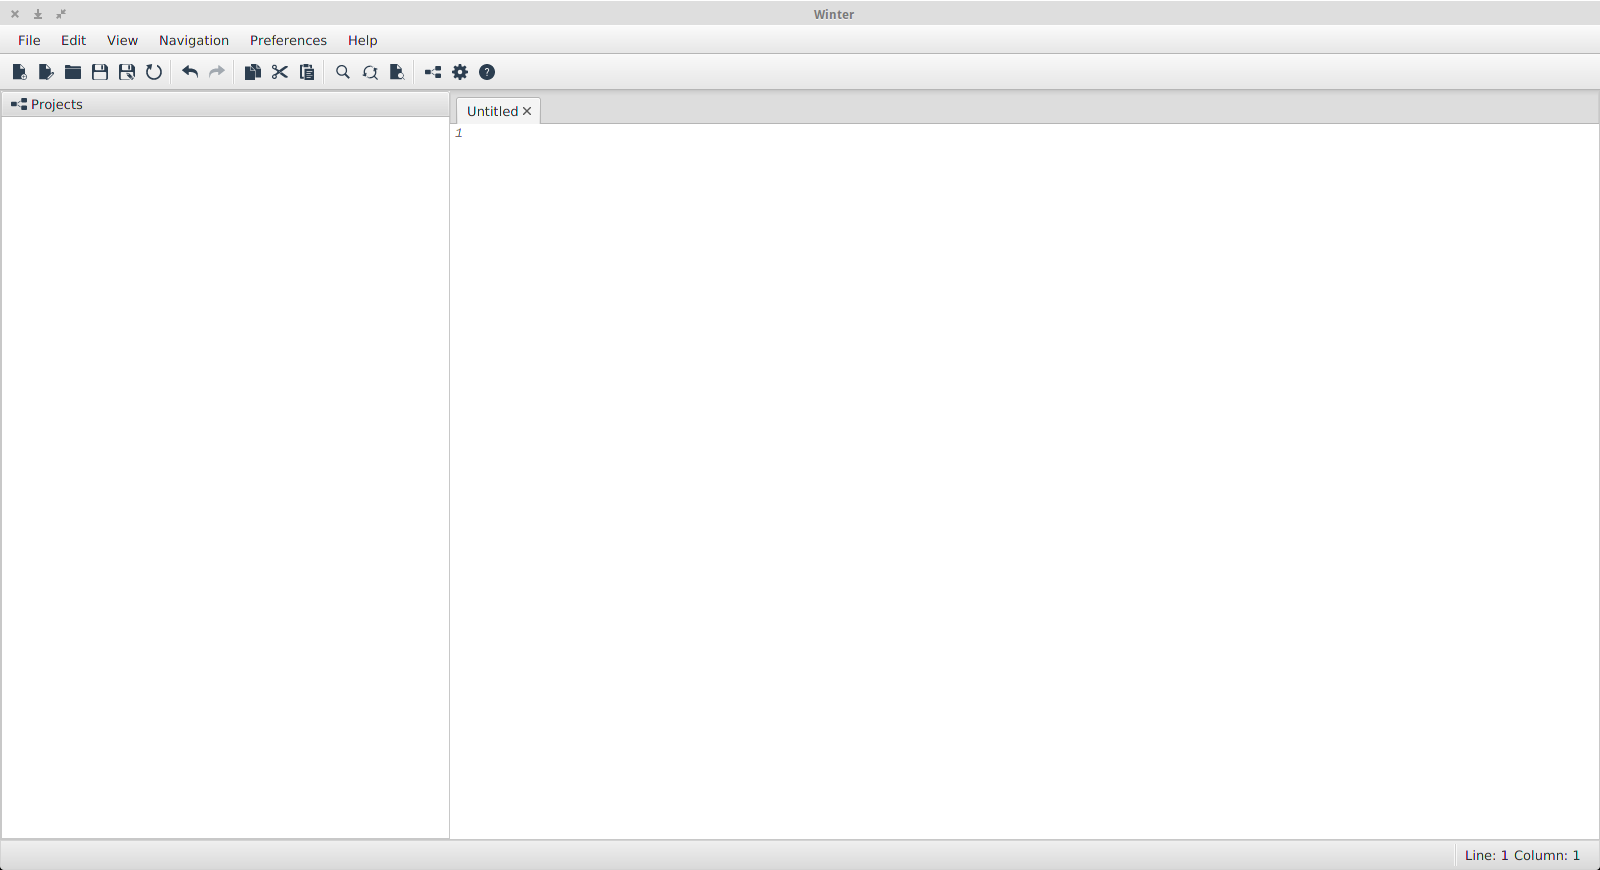
\includegraphics[width=\textwidth]{winter}
\caption{The Winter text editor}
\centering
\end{figure}

That's it. Installing Winter simply means downloading the jar file.

Note that you can't run both the Meruem interpreter (we can also just refer to it simply as "Meruem") and Winter by installing Java first.

\section{Running the REPL}
Many programming languages like Scala, Haskell, Clojure (another Lisp that runs on the JVM), Python, Ruby, and more, have what is known as a REPL. A \ikeyword{REPL} (Read-Eval-Print-Loop), also known as \keyword{interactive shell}, is a program that reads input from the user (Read), evaluate it (Eval), prints the result (Print) and ask for another input (Loop). Every Lisp has a REPL (as far as I know). And since Meruem is a Lisp, it has a REPL too. It's called The Meruem REPL (surprise!). 

The Meruem REPL is already packaged with the Meruem distribution that you have downloaded earlier. To run it, first, fire up the terminal (or command prompt, but from now on we'll just refer to it as "Terminal"). Then use the \code{cd} command to go to the directory where you installed Meruem. (If you don't want to keep on doing the previous step, you can add the path to Meruem's installation directory to your environment paths). When you're already inside the installation directory, just type \code{java -jar meruem.jar} and press the enter key. You should be able to see the following on the terminal:

\begin{REPL}
meruem>
\end{REPL}

This signifies that the REPL has successfully started and that it is waiting for you to enter something. Try entering the expression \code{(+ 1 2)}, and then press enter:

\begin{REPL}
meruem> (+ 1 2)
3
meruem>
\end{REPL}

The answer \code{3} has been printed. Now the REPL is waiting for another input. Don't worry if you don't understand what the code \code{(+ 1 2)} does. For now, what's important is to confirm that your REPL works fine.

To exit the REPL, run \code{exit}:

\begin{REPL}
meruem> exit
Bye!
\end{REPL}

The REPL is useful if all you want to do is to try out some expressions. Instead of creating a new source file for that, you can just evaluate things inside the interactive shell and immediately see the results of the evaluations.

\section{Hello World in Meruem}
\label{sec:helloworld}
It is almost customary for any programming language tutorial to have a \code{Hello World} program as the very first complete program to run. We are going to follow such practice here.

First, run Winter (again by running the \code{java -jar Winter.jar} command.). Next, type the following in the editor area:

\begin{Meruem}
(defun main (args) (println "Hello World"))
\end{Meruem}

Save it as \code{hello\_world.mer}. Then, \code{cd} into where you saved \code{hello\_world.mer} and run the following command: \code{java -jar meruem.jar hello\_world}. You should be able to see the following output:

\begin{REPL}
$ java -jar meruem.jar hello_world
Hello World
\end{REPL}

The \code{hello\_world} is the name of the source file you want to run. Basically, if the source file is not provided, Meruem will fire up the REPL for you. 

If the code worked, then congratulations, you've just run your first complete Meruem program. This also means that your set up is complete and working well. Now you are ready to start learning the Meruem programming language.